\chapter{The Hypercompressor}
\label{ch:hypercompressor}

The idea for Hypercompression came during the development of Vocal
Vibrations.\cite{Holbrow2014} What if we could position audio in space
as carefully and maticulously as we can position audio in time?

\section{Ambisonics}
\label{sec:ambisonics}
Ambisonic audio is a technique for encoding and decoding three-dimensional
surround sound audio.\cite{Gerzon1985} Ambisonics differs from other
surround sound formats like $5.1$ and $7.1$ in that it does not depend
on a particular speaker configuration. An ambisonic recording can be
decoded on any surround sound speaker configuration without
disarranging the spatial contents of the audio recording.

Immagine we used an omnidirectinoal microphone to record an acoustic
instrument at a sample rate of $44.1$ kHz. We sample and record 44100
samples every second that represent the air pressure at the microphone
capsule during the recording. Our omni-directional microphone is
designed to treat sound arriving from all angles equally. The
omnidirectional microphone sums together sounds arriving from all
angles and the acoustic directional information is lost.

If we want to encode, decode, transmit, or play audio that preserves
full sphere 360 degree information, ambisonics offers a solution.
Ambisonic audio uses \textit{spherical harmonics} to encode surround
sound audio that preserves the direction-of-arrival information that
discrete channel recordings (such as mono and stereo) cannot fully
capture.

\subsection{Spherical Harmonics}
\label{sec:spherical-harmonics}
We know that we can construct any monophonic audio waveform by summing
a (possibly infinite) number harmonic sine waves (fourier
series).\sidenote{An excelent description of the transormation between
  the time domain and frequency domain can be fount at
  \url{http://betterexplained.com/articles/an-interactive-guide-to-the-fourier-transform/}}
For example, by summing odd \textit{order} sine harmonics at a given
frequency $f$, $(1f, 3f, 5f, 7f, \ldots )$, we generate a square wave with
fundamental frequency $f$. As the order increases, so does the
temporal resolution of our square wave.

By summing sinusoidal harmonics, we can generate any continuous
waveform defined in two dimensions (one input parameter and one
output). Similarly, by summing \emph{spherical harmonics}, we can
generate any continous shape defined over the surface of a
three-dimensional sphere (two input parameres, or polar angles, one
output). Where a traditional monophonic audio encoding might save one
sample 44100 times per second, an ambisonic encoding would save one
sample \emph{for each spherical harmonic} 44100 times per second. This
way we capture a three-dimensional sound image at each audio sample.
The number of spherical harmonics we encode is determined by our
\textit{ambisonic order}. As our ambisonic order increases, so does
the angular resolution of our result on the surface of the sphere.

\subsection{Spherical Harmonic Definition}
For encoding and decoding ambisonics, the convention is to use the
real portion of spherical harmonics as defined in
equation~\ref{eq:spherical}, where:
\begin{itemize}
\item $Y_{n}^{m}(\varphi,\vartheta)$ is a spherical harmonic that
is:\marginnote{Some literature on spherical harmonics swaps the names
  of\textit{order} and \textit{degree}. In this thesis we use
  $Y_{order}^{degree}$. In literature where $Y_{degree}^{order}$ is
  used, the function of the subscript and superscript remain
  unchanged; only the names are inconsistent.}
\begin{itemize}
\item of order, $n$
\item of degree, $m$
\item defined over spherical coordinates $(\varphi, \vartheta)$
\end{itemize}
\item $N_n^{|m|}$ is a normalization factor.\sidenote{In ambisonic
    literature (and software), there are multiple incompatible
    conventions for the normalization of spherical harmonics. This
    thesis asumes the SN3D convention as recomended by the AMBIX
    format specification.}\cite{Nachbar2011}
\item $P_n^{|m|}$ is the associated Legendre function of order $n$,
  and degree $m$.
\end{itemize}
\begin{equation}
Y_{n}^{m}(\varphi,\vartheta)=N_n^{|m|}P_n^{|m|}(\sin{\vartheta})
\begin{cases}\label{eq:spherical}
\sin{|m|\varphi},&  \text{for $m<0$}\\  
\cos{|m|\varphi},& \text{for $m\geq 0$}\\
\end{cases}
\end{equation}
Given equation~\ref{eq:spherical}, we can define an ambisonic
audio recording as:
\begin{equation}
f(\varphi,\vartheta,t)=\sum\limits_{n=0}^N\sum\limits_{m=-n}^nY_n^m(\varphi,\vartheta)\phi_{nm}(t)
\label{eq:ambisonics}
\end{equation}
Where:
\begin{itemize}
\item $\varphi$ and $\vartheta$ describe the polar angle of sound
  arrival in two dimensions.\sidenote{Note that ambisonics uses polar
    angles to describe the angle of arrival of sound. These are
    similar to spherical coordinates, minus the inclusion of
    \textit{radial distance}. Distance is not part of the ambisonic
    specification.}
\item $t$ is time
\item $\phi_{nm}(t)$ are our \textit{expansion coeficients}, described
  below.
\end{itemize}
\begin{figure}[]
  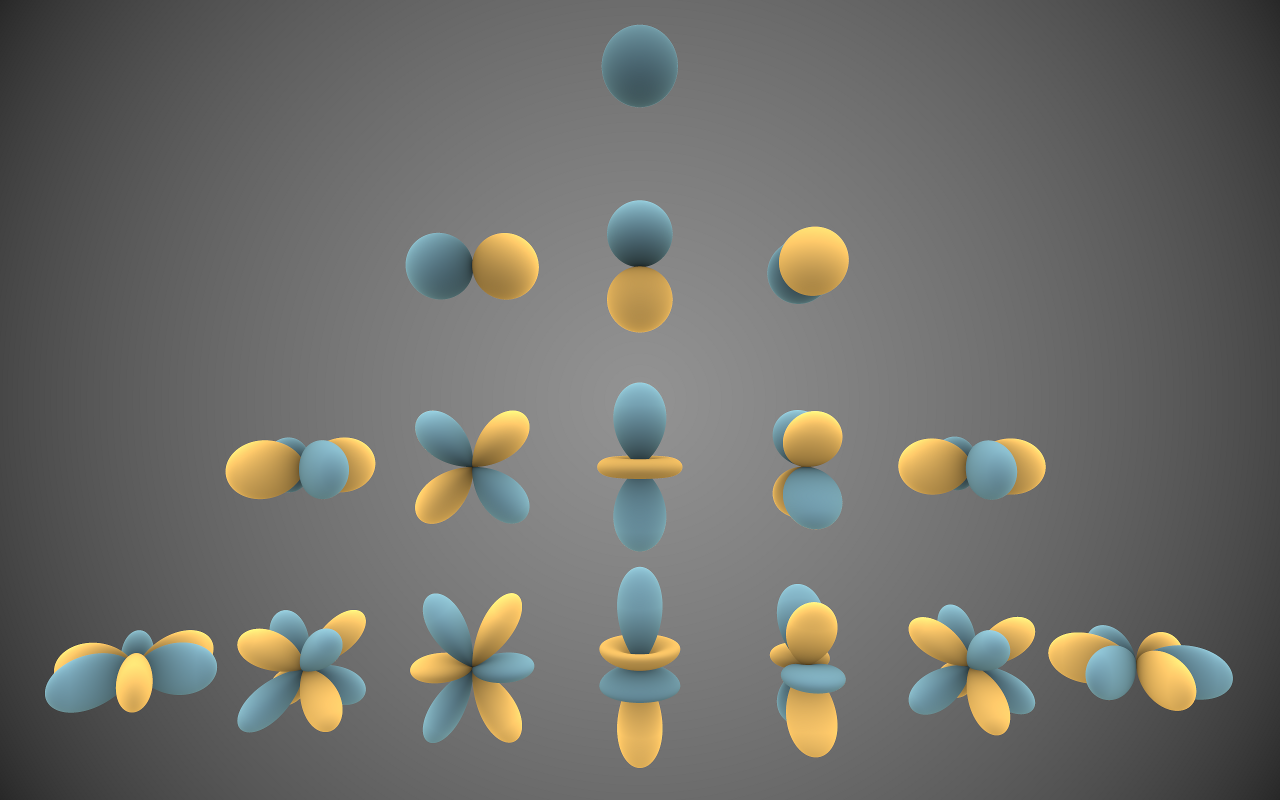
\includegraphics[width=\linewidth]{SphericalHarmonics.png}
  \caption{Spherical harmonics $0$th order (top row) through $3$rd
    order (bottom row). This for image shows the output of
    $Y_{n}^{m}(\varphi,\vartheta)$ for $n=0,n=1,n=2,$and $n=3$. The
    distance of the surface from the origin shows the value at that
    angle. Darker blue regions are positive, while lighter yellow
    regions are negative. Image credit: Ingo Quilez, licensed under
    \textit{Creative Commons Attribution-Share Alike 3.0 Unported}.}
  \label{fig:spherical-harmonics}
\end{figure}

\subsection{Spherical Harmonic Expansion Coeficients}
\label{sec:spher-harm-expans}
In our monophonic recording example, we save just one digital sample
44100 times per second, with each saved value representing the air
pressure at a point in time. We know that by summing the correct
combination of spherical harmonics, we can describe any continous
function over the surface of a sphere. Instead of sampling air
pressure directly, we sample a coefficient describing the weighting of
each spherical harmonic 44100 times per second. The resulting sphere
encodes the pressure including the direction of arrival
information. The weighting coefficients or \textit{expansion
  coefficients} are recorded in our audio file instead of values
representing air pressure directly. Now, by summing together our
weighted spherical harmonics, we can reconstruct the fluctuations in
pressure including the angle of arrival information. We can recall
this snapshot of information 44100 times per second.

\subsection{Usage}
\label{sec:usage}
There are two ways to create an ambisonic recording. First, we can use
a soundfield microphone to record an acoustic soundfield. Soundfield
microphones like the one developed by Calrec Audio can capture angle
of arrival information with the spatial resolution of first order
ambisonics.\cite[-1in]{Ferrar1979} Alternativley, we can algorithmically
encode pre-recorded sources to create a virtual sources in an
ambisonic bus.\cite[-0.4in]{Malham1995}

\section{Building on the Compression Paradigm}
\marginnote{Unless noted otherwise, ``compression'' is used in this
  thesis to describe dynamic range compression, as opposed to data
  compression.}  The design, implementation, and use of traditional
dynamic range compression is well documented in
literature,\cite[7mm]{Giannoulis2012,Case2007,Deruty2014} so the we will
describe dynamic range compression only as much as is needed to
explain the foundation for \thesis. Immagine we are
mixing a vocal pop performance, and during the verse, and our singer
is singing moderately loud, or \textit{mezzo-forte}. At the beginning
of the chorus, our singer wants a full and powerful sound, so she
adjusts the dynamic to very loud, or \textit{fortissimo}. However, the
new louder dynamic interrupts the balance between the vocals and the
other instruments in our mix. We like the powerful sound of our
singer's \textit{fortissimo} performance, but our balance would be improved
if we had the volume of a \textit{forte} performance instead. One option is to
manually turn down the vocalist during the chorus, and in some cases
this is the best solution. When we want more precise control, we can
use a compressor.

\subsection{Traditional Compression}
\label{sec:trad-compr}
A compressor is essentially an automated dynamic volume control. We
send our vocalist's audio signal through a compressor, and whenever
her voice exceedes a set \textit{threshold}, the signal is
automatically attenuated. As the input signal further exceeds the
level set by our compressors' threshold parameter, the output is
further attenuated relative to the input signal. The compressor
includes a \textit{ratio} parameter that determines the relationship
between the input level and output level as shown in
figure~\ref{fig:comp-ratio}.

\begin{marginfigure}
  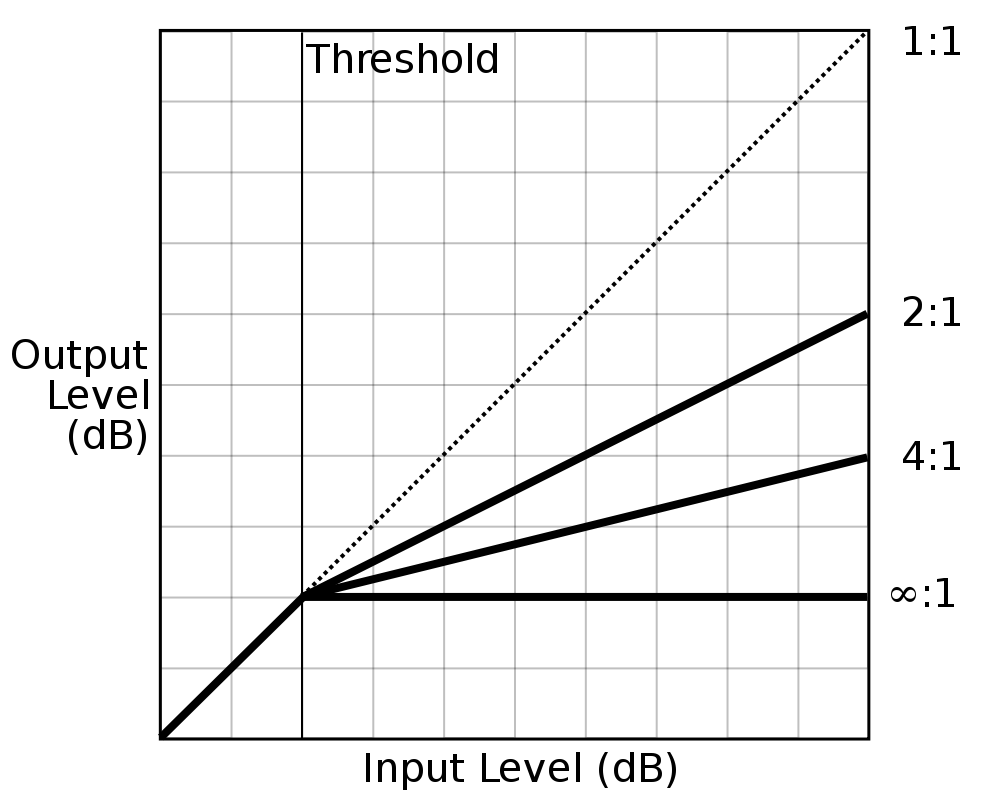
\includegraphics[]{CompressionRatio.png}
  \caption{``Compression ratio'' by Iain Fergusson. Licensed under
     Public Domain via Wikimedia Commons 
     \url{https://commons.wikimedia.org/wiki/File:Compression_ratio.svg\#/media/File:Compression_ratio.svg}
   }
  \label{fig:comp-ratio}
\end{marginfigure}

The threshold and ratio parameters are essential for controling dynamic
range, but the power and creative flexibility of the compressor comes
with two additional input parameters: \textit{attack time}, and
\textit{release time}. These parameters determine the speed at which
the compressor attenuates (attack) and disengages (release) when the
input signal exceeds the threshold. By adjusting the attack and
release times, we can change the focus of the compressor.
\begin{itemize}
\item Perhaps we want the compressor to engage or disengage at the
  time scale of a musical phrase. We could set our attack time long
  enough to let transients through without engaging the compressor
  significantly (try 20 miliseconds). If our relsease time is quite
  long (try 300 milliseconds), and we set our threshold and ratio
  carefully, we might be able to convince the compressor to smooth
  musical phrases.
\item If we want our compressor to focus on syllables instead of
  phrases, we can shorten our attack and release times (try 10
  milliseconds and 40 milliseconds respecrively). When the compressor
  engages and disengages at each syllable, it imparts a different
  quality (sometimes described as ``punch'').
\item If we reduce our attack and release parameters enough, we can
  instruct our compressor to engage and disengage at the time scale of
  an audio waveform, compressing individual cycles. This will distort
  an audio signal, adding odd order harmonics,\sidenote{Not every
    compressor model can react quickly enough to distort a waveform. The Dbx
  160 and Teletronix LA2A are known to be fast enough to distort.} and
imparting an entirely different quality.
\end{itemize}
The attack and release times listed here are a rough guide only.  The
exact function of these parameters varies from one model of compressor
to another, and results also depend on the audio input material, and
on the threshold and ratio settings. Again, the results of audio
compression can sometimes be characterized better by a feeling than a
formula.

\section{An Ambisonic Compressor}
\label{sec:ambis-compr}
In the 

\begin{figure*}
  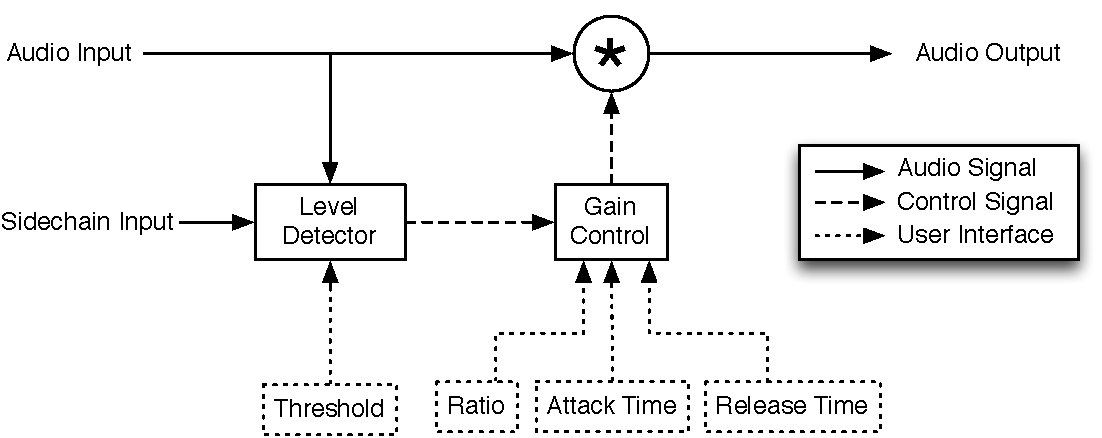
\includegraphics[width=\linewidth]{SimpleCompressor.pdf}
  \caption{Block diagram of a simple traditional dynamic range
    compressor.}
  \label{fig:comp-block}
\end{figure*}


%%% Local Variables:
%%% mode: latex
%%% TeX-master: "CharlesHolbrow_MAS_Thesis"
%%% End:
